%%%%%%%%%%%%%%%%%%%%%%%%%%%%%%%%%%%%%%%%%%%%%%%%%%%%%%%%%%%%%%%%%%%%%%%%%%%%
% AGUJournalTemplate.tex: this template file is for articles formatted with LaTeX

%% To submit your paper:
\documentclass[draft]{agujournal2019}
\usepackage{url} %this package should fix any errors with URLs in refs.
\usepackage{lineno}
\usepackage[colorlinks=true, urlcolor=blue, linkcolor=red]{hyperref}
\usepackage{minted}
\usepackage{natbib}
\usepackage{subfiles}
\usepackage{xr}
\usepackage[inline]{trackchanges} %for better track changes. finalnew option will compile document with changes incorporated.
\usepackage{soul}

\linenumbers

\draftfalse

\journalname{Geophysical Research Letters}

%----Helper code for dealing with external references----
% (by cyberSingularity at http://tex.stackexchange.com/a/69832/226)

\usepackage{xr}
\makeatletter

\newcommand*{\addFileDependency}[1]{% argument=file name and extension
\typeout{(#1)}% latexmk will find this if $recorder=0
% however, in that case, it will ignore #1 if it is a .aux or 
% .pdf file etc and it exists! If it doesn't exist, it will appear 
% in the list of dependents regardless)
%
% Write the following if you want it to appear in \listfiles 
% --- although not really necessary and latexmk doesn't use this
%
\@addtofilelist{#1}
%
% latexmk will find this message if #1 doesn't exist (yet)
\IfFileExists{#1}{}{\typeout{No file #1.}}
}\makeatother

\newcommand*{\myexternaldocument}[1]{%
\externaldocument{#1}%
\addFileDependency{#1.tex}%
\addFileDependency{#1.aux}%
}
%------------End of helper code--------------

% put all the external documents here!
\myexternaldocument{supplement}
\begin{document}
%TC:ignore
%% ------------------------------------------------------------------------ %  TITLE
%% ------------------------------------------------------------------------ 
\title{Land Processes Can Substantially Impact the Mean Climate State
}

%% ------------------------------------------------------------------------ 
%  AUTHORS AND AFFILIATIONS
%% ------------------------------------------------------------------------ 

\authors{Claire M. Zarakas\affil{1} , 
Daniel Kennedy\affil{3}, 
Katherine Dagon\affil{3}, 
David M. Lawrence\affil{3}, 
Amy Liu\affil{1}, 
Gordon Bonan\affil{3}, 
Charles Koven\affil{4},
Danica Lombardozzi\affil{3},
and Abigail L. S. Swann\affil{1,2}}

\affiliation{1}{University of Washington, Department of Atmospheric Sciences}
\affiliation{2}{University of Washington, Department of Biology}
\affiliation{3}{National Center for Atmospheric Research}
\affiliation{4}{Lawrence Berkeley National Laboratory}

%% Corresponding Author:
\correspondingauthor{Claire M. Zarakas}{czarakas@uw.edu}

%% ------------------------------------------------------------------------ 
%  Keypoints (final entry on title page)
%% ------------------------------------------------------------------------ 

%  List up to three key points (at least one is required)
%  Each must be 140 characters or fewer with no special characters or punctuation and must be complete sentences

\begin{keypoints}
\item Assumptions about land processes substantially impact mean state terrestrial temperature and precipitation.
\item Land parameters influence climate predominantly through changing evapotranspiration rather than through other mechanisms.
\item Warming driven by land processes activates different atmospheric feedbacks than radiatively-driven warming.
\end{keypoints}
%TC:endignore
%% ------------------------------------------------------------------------
%  ABSTRACT and PLAIN LANGUAGE SUMMARY
%% ------------------------------------------------------------------------

\begin{abstract}
Terrestrial processes influence the atmosphere by controlling land-to-atmosphere fluxes of energy, water, and carbon. Prior research has demonstrated that parameter uncertainty drives uncertainty in land surface fluxes. However, the influence of land process uncertainty on the climate system remains underexplored. Here, we quantify how assumptions about land processes impact climate using a perturbed parameter ensemble for 18 land parameters in the Community Earth System Model (CESM2) under preindustrial conditions. We find that an observationally-informed range of land parameters generate biogeophysical feedbacks that significantly influence the mean climate state, largely by modifying evapotranspiration. Global mean land surface temperature ranges by 2.2°C across our ensemble ($\sigma$ = 0.5°C) and precipitation changes were significant and spatially variable. Our analysis demonstrates that the impacts of land parameter uncertainty on surface fluxes propagates to the entire Earth system, and provides insights into where and how land process uncertainty influences climate.
\end{abstract}

\section*{Plain Language Summary}
Land processes can affect climate by controlling the transfer of energy and water from the land to the atmosphere. Previous research has shown that uncertainty surrounding land processes (e.g. photosynthesis and the movement of water through soils) can drive uncertainty in land-to-atmosphere fluxes. However, it remains unclear how much that land uncertainty can impact climate. Here, we quantify how climate is sensitive to assumptions about land processes by varying 18 land model parameters to create an ensemble of 36 possible worlds in a global climate model. Land temperature ranges by 2.2°C across this ensemble, mostly due to changes in how much water is evaporated from the land surface. Changing land parameters also drives regionally variable changes in mean precipitation. This study highlights a large and underappreciated impact of land processes in determining the mean climate state, and provides insights into how climate is influenced by land process uncertainty.

%% ------------------------------------------------------------------------ 

\section{Introduction}

Land models were initially developed to support weather and climate prediction by providing atmospheric models with lower boundary conditions of energy, water, and momentum fluxes. Given this limited scope, early land models were simple biogeophysical models, in which land-to-atmosphere fluxes were determined by prescribed land surface albedo, evaporative resistance, and roughness \citep{manabe_climate_1969}. Since then, land models have substantially expanded in scope and complexity. Modern land models now represent biogeochemical cycling, hydrology, ecology, land use, and land management, and are used to predict how processes across these domains interact and respond to global change \citep{fisher_perspectives_2020}. This evolution has been accompanied by an increase in the number of model parameters, many of which can influence land-to-atmosphere fluxes by altering the emergent land surface albedo, turbulent flux partitioning, and roughness.

The increasingly complex land model parameter space has driven a large body of research exploring the implications of land parameter uncertainty for land model calibration \citep{dagon_machine_2020}, carbon and water flux uncertainty quantification \citep{hou_sensitivity_2012,mcneall_constraining_2023}, and process understanding \citep{boulton_exploring_2017}. Earth system parametric uncertainty is often quantified through perturbed parameter ensembles (PPEs), in which multiple poorly constrained parameters are systematically varied within a single model structure. Land PPEs have demonstrated that parameter uncertainty is a major driver of uncertainty in land-to-atmosphere surface fluxes, at local \citep{ricciuto_impact_2018,fisher_parametric_2019}, regional \citep{bauerle_carbon_2014,huo_parameter_2019}, and global scales \citep{dagon_machine_2020,zaehle_effects_2005}.

%\hl{(Duan et al. 2018, Raczka et al., 2018, Viskari et al., 2019, Shiklomanov et al. 2020, Yuan et al. 2023, Chen et al. 2023, TK more})

Most existing land parameter uncertainty studies have quantified parameters’ impact in a land-only framework \citep{zaehle_effects_2005, dagon_machine_2020, ricciuto_impact_2018, bauerle_carbon_2014, fisher_parametric_2019, dietze_quantitative_2014, bauerle_carbon_2014}, where the atmospheric forcing is an external boundary condition and land surface fluxes do not influence the atmosphere. Only a handful of previous studies have assessed the biogeophysical \citep{liu_constraining_2005,fischer_quantifying_2011,williams_land-atmosphere_2016} or carbon cycle \citep{booth_high_2012, booth_narrowing_2017, hawkins_parametric_2019, mcneall_constraining_2023} implications of land parameter uncertainty in a coupled context, or included land parameters in PPEs perturbing parameters across the Earth system \citep{sexton_perturbed_2021, yamazaki_perturbed_2021}. This is in part due to computing constraints. For example, in the Community Earth System Model version 2 (CESM2), a simulation with a dynamic atmosphere requires about ten times more computing time per modeled year than a land-only simulation, and coupled configurations often require more simulated years to establish a signal due to internal variability of the coupled system \citep{kay_community_2015}. Additionally, the prevalence of land-only analyses reflects the land modeling community’s focus on how land parameter uncertainty influences terrestrial processes, rather than atmospheric processes. The biogeophysical impact of land parameter uncertainty on atmospheric processes and land-atmosphere interactions remains underexplored. Of the few studies which have assessed land parameter uncertainty in a coupled context, only one has quantified the biogeophysical impact of land parameters on climate globally \citep{fischer_quantifying_2011}.

This is a problematic gap in the literature because land parameters’ demonstrated influence on land surface fluxes suggests that land parameters can influence the mean climate state. It has been established for decades that changes in land surface albedo \citep{charney_drought_1975, charney_dynamics_1975, charney_comparative_1977}, roughness \citep{sud_influence_1988}, and capacity to evaporate water \citep{shukla_influence_1982} can alter temperature and precipitation on global scales. More recently, \cite{lague_separating_2019} used a modern Earth system model to show that atmospheric feedbacks are critical in determining how land temperatures respond to idealized land surface changes. Extensive previous work has demonstrated that changes in land cover can drive local, regional, and remote climate impacts \citep[e.g.][]{pongratz_biogeophysical_2010,swann_mid-latitude_2012,boysen_global_2020}. Additionally, changing land model representations of terrestrial processes such as stomatal conductance and soil hydrology can influence the mean climate state \citep{lawrence_partitioning_2007} and frequency of extremes \citep{kala_impact_2016}.

In this study, we aim to close this gap in the literature by using a coupled PPE to address the following questions: (1) to what extent can land parameters impact the mean climate state? and (2) through what mechanisms do land parameters influence climate?

%% ------------------------------------------------------------------------ 
\section{Methods}
%\subsection{Model configurations}
We ran PPEs under preindustrial conditions using two configurations of CESM2 \citep{danabasoglu_community_2020}: a partially coupled configuration (“coupled”) and an uncoupled, land only configuration (“land-only”). In both the coupled and land-only PPE, the land model \citep[the Community Land Model version 5, CLM5;][]{lawrence_community_2019} was run with prognostic leaf area. In the coupled ensemble, we ran preindustrial simulations with constant greenhouse gas concentrations using an active atmosphere \citep[CAM6;][]{bogenschutz_path_2018} and a slab ocean \citep{danabasoglu_equilibrium_2009}. Because these simulations have fixed concentrations of greenhouse gasses including CO$_2$, they capture the biogeophysical impacts of land parameters which is the focus of this paper, but they do not capture biogeochemical feedbacks. The land-only simulations used a custom atmospheric forcing, which was generated by CAM6 in the reference coupled simulation that used default parameters.

%\subsection{Perturbed parameter ensemble design}
Our PPEs sampled 18 land parameters (Table S\ref{table:param_list}), and our parameter selection was informed by the CLM5 PPE project (data and methods description are available via \url{https://github.com/djk2120/clm5ppe}). The CLM5 PPE differs from ours in that the simulations were run in a land-only configuration forced with observationally-derived atmospheric data for present-day. Nonetheless, the one-at-a-time parameter perturbations provide insight into which parameters might be meaningful for our coupled PPE. We used two parameter selection criteria: (1) that parameters would likely have a large impact on the atmosphere, based on results from the CLM5 PPE, and (2) that parameters sampled different functional areas of the model (\ref{Text:parameter_selection}). The 18 parameters we selected are described in detail in Table S\ref{table:metrics_of_impact} and span nine functional categories: soil hydrology, stomatal conductance and plant water use, snow, photosynthesis, boundary layer / roughness, radiation, canopy evaporation, biomass heat storage, and temperature acclimation.

For each parameter, we ran two simulations, where the parameter was perturbed to a minimum and maximum value (ensemble n = 36). We used the parameter ranges from the CLM5 PPE, which were determined by domain-area experts based on literature review and expert judgement. Because some parameters have larger ranges than others, our analysis includes both the sensitivity of the climate system to a change in a parameter combined with the uncertainty in that parameter’s range. We note that this one-at-a-time sampling procedure does not account for parameter interactions, though we expect that parameter interactions may be of second-order importance based on \cite{fischer_quantifying_2011} who finds that nonlinear interactions between parameters were minimal in a stationary climate.

%% ------------------------------------------------------------------------ 
\section{Results and Discussion} 
%% ------------------------------------------------------------------------ 
\subsection{Mean temperature changes}
Our ensemble demonstrates that land parameters can substantially impact the mean climate state. Global mean land surface temperatures range by 2.2°C across our coupled PPE ($\sigma$ = 0.5°C), and by over 3°C at some latitudes ($\sigma$ $>$ 0.65°C above 67°N; Figure ~\ref{fig:temperature_changes}a). Seven out of 18 parameters generated a greater than 1°C temperature range (Figure ~\ref{fig:temperature_changes}b), and more than 70$\%$ of the land surface experienced statistically significant changes in annual mean temperature in 20 out of the 36 ensemble members (Figure S\ref{fig:supp_coupled_Ts_land_maps}). Global mean surface temperatures (including ocean) ranged by 1.1°C ($\sigma$ = 0.5°C; Figure S\ref{fig:supp_coupled_Ts_land_and_ocean_maps}- S\ref{fig:supp_coupled_Ts_land_vs_ocean_maps}), which is over 40$\%$ of the preindustrial absolute temperature range in CMIP6 \citep[2.4°C, $\sigma$=0.58°C;][]{tett_does_2022} and CMIP5 \citep{hawkins_connecting_2016}. Three soil hydrology parameters - \mintinline{Fortran}{frac_sat_soil_dsl_init}, \mintinline{Fortran}{d_max}, and \mintinline{Fortran}{fff} - had the largest impact on global mean temperature. Land surface temperature changes in the land-only PPE were generally much smaller than those in the coupled PPE (Figure ~\ref{fig:temperature_changes}), consistent with the fact that atmospheric feedbacks substantially amplify the land surface temperature response to changing land surface properties \citep{lague_separating_2019}.

\begin{figure}
\noindent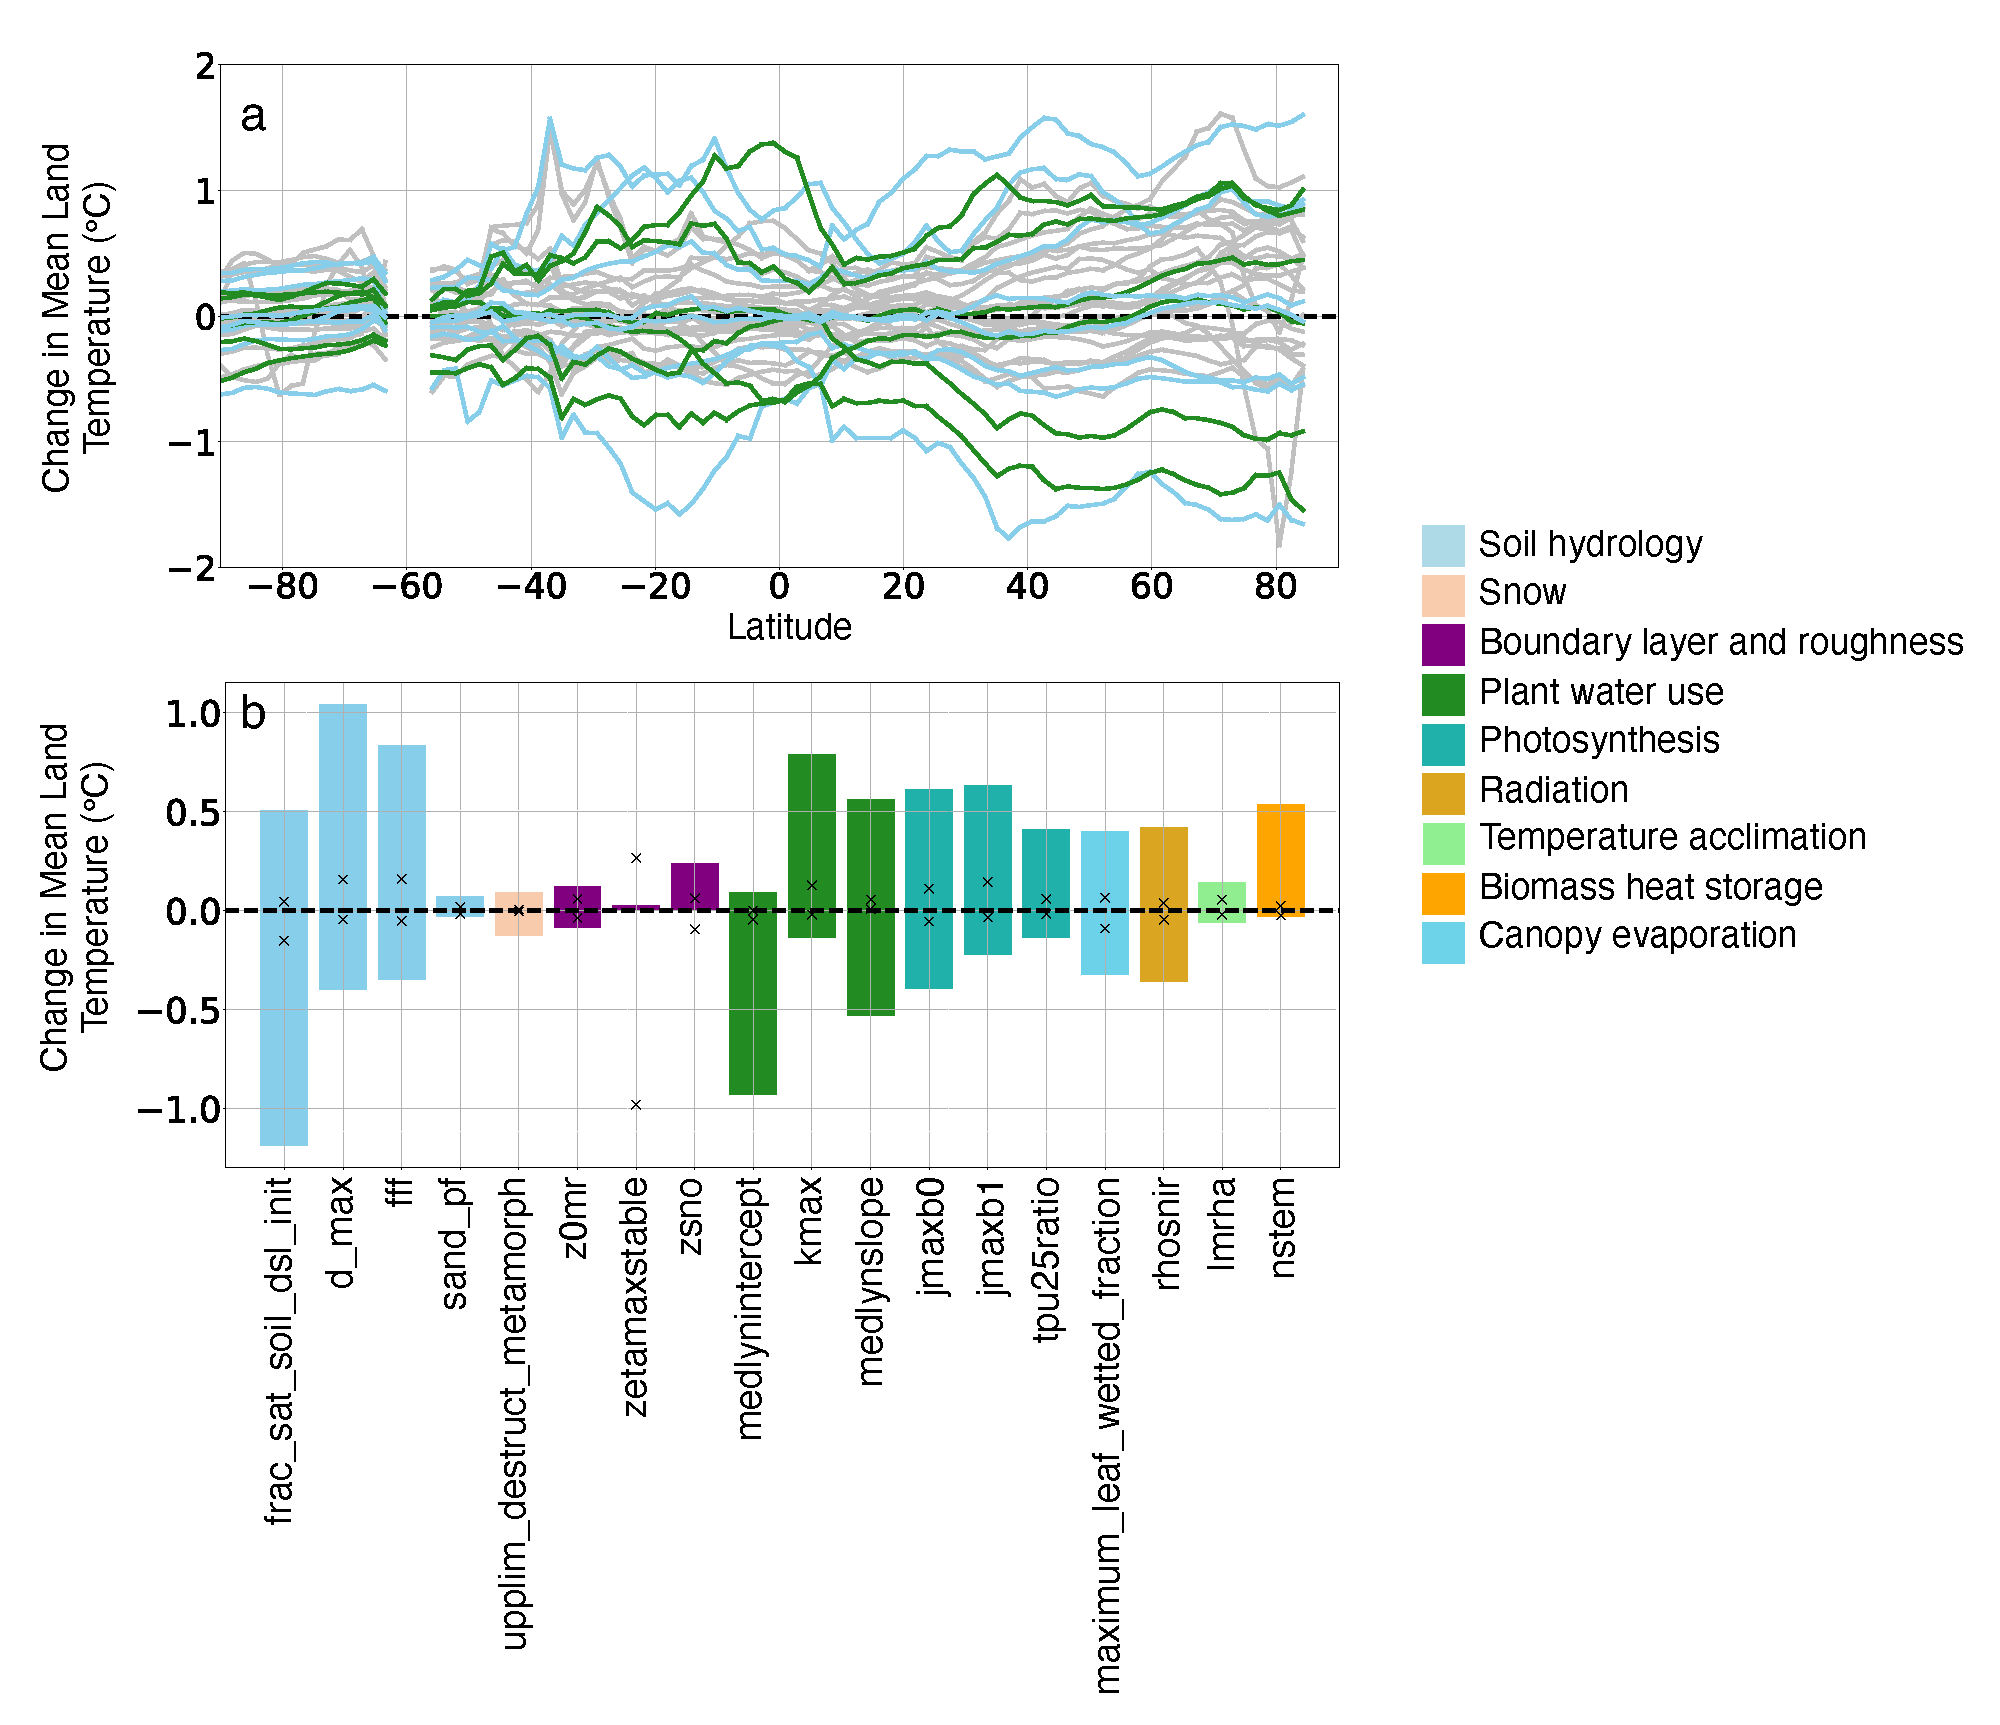
\includegraphics[width=\textwidth]{figs/Figure1.pdf}
\caption{Zonal mean (a) and global mean (b) changes in annual land temperature across the coupled PPE, relative to the default simulation. Color indicates parameter category, and only ensemble members perturbing soil hydrology and plant water use parameters are colored in (a). In (b), bars indicate the range of coupled global mean land surface temperature changes associated with each parameter, and Xs mark the range of land-only global mean land surface temperature changes.}
\label{fig:temperature_changes}
\end{figure}

Parameters generally impacted surface temperature with a similar spatial pattern globally. The leading mode of variability in annual mean surface temperature changes, as quantified by the first empirical orthogonal function \citep[EOF; ][]{lorenz_empirical_1956}, explains 78$\%$ of the variance across our coupled ensemble (Figure \ref{fig:temperature_patterns}a, Figure S\ref{fig:supp_EOF_analysis_Temp}) and is highly correlated with the global average mean land temperature change (Figure S\ref{fig:supp_EOF_globalmetric_correlation}). As expected, the leading EOF in the land-only ensemble explains less of the temperature variance and has a different spatial pattern (Figure ~\ref{fig:temperature_patterns}b), indicating that regional to global-scale atmospheric responses contribute to the consistent coupled PPE pattern of temperature change. Notably, the leading coupled PPE EOF differs from the typical pattern of radiatively driven warming (e.g. CO$_2$-driven warming, Figure ~\ref{fig:temperature_patterns}c and \ref{Text:doubling_CO2}), a pattern which is generally consistent across climate models (Proistosescu et al. 2020). This indicates that the dominant coupled spatial pattern is not only due to parameter-driven temperature changes kicking off radiative feedbacks (e.g. ice albedo feedback, water vapor feedback) which have consistent spatial fingerprints. Rather, this suggests that land parameter uncertainty drives a consistent temperature response pattern, despite the fact that parameters influence different terrestrial processes.

\begin{figure}
\centering
\noindent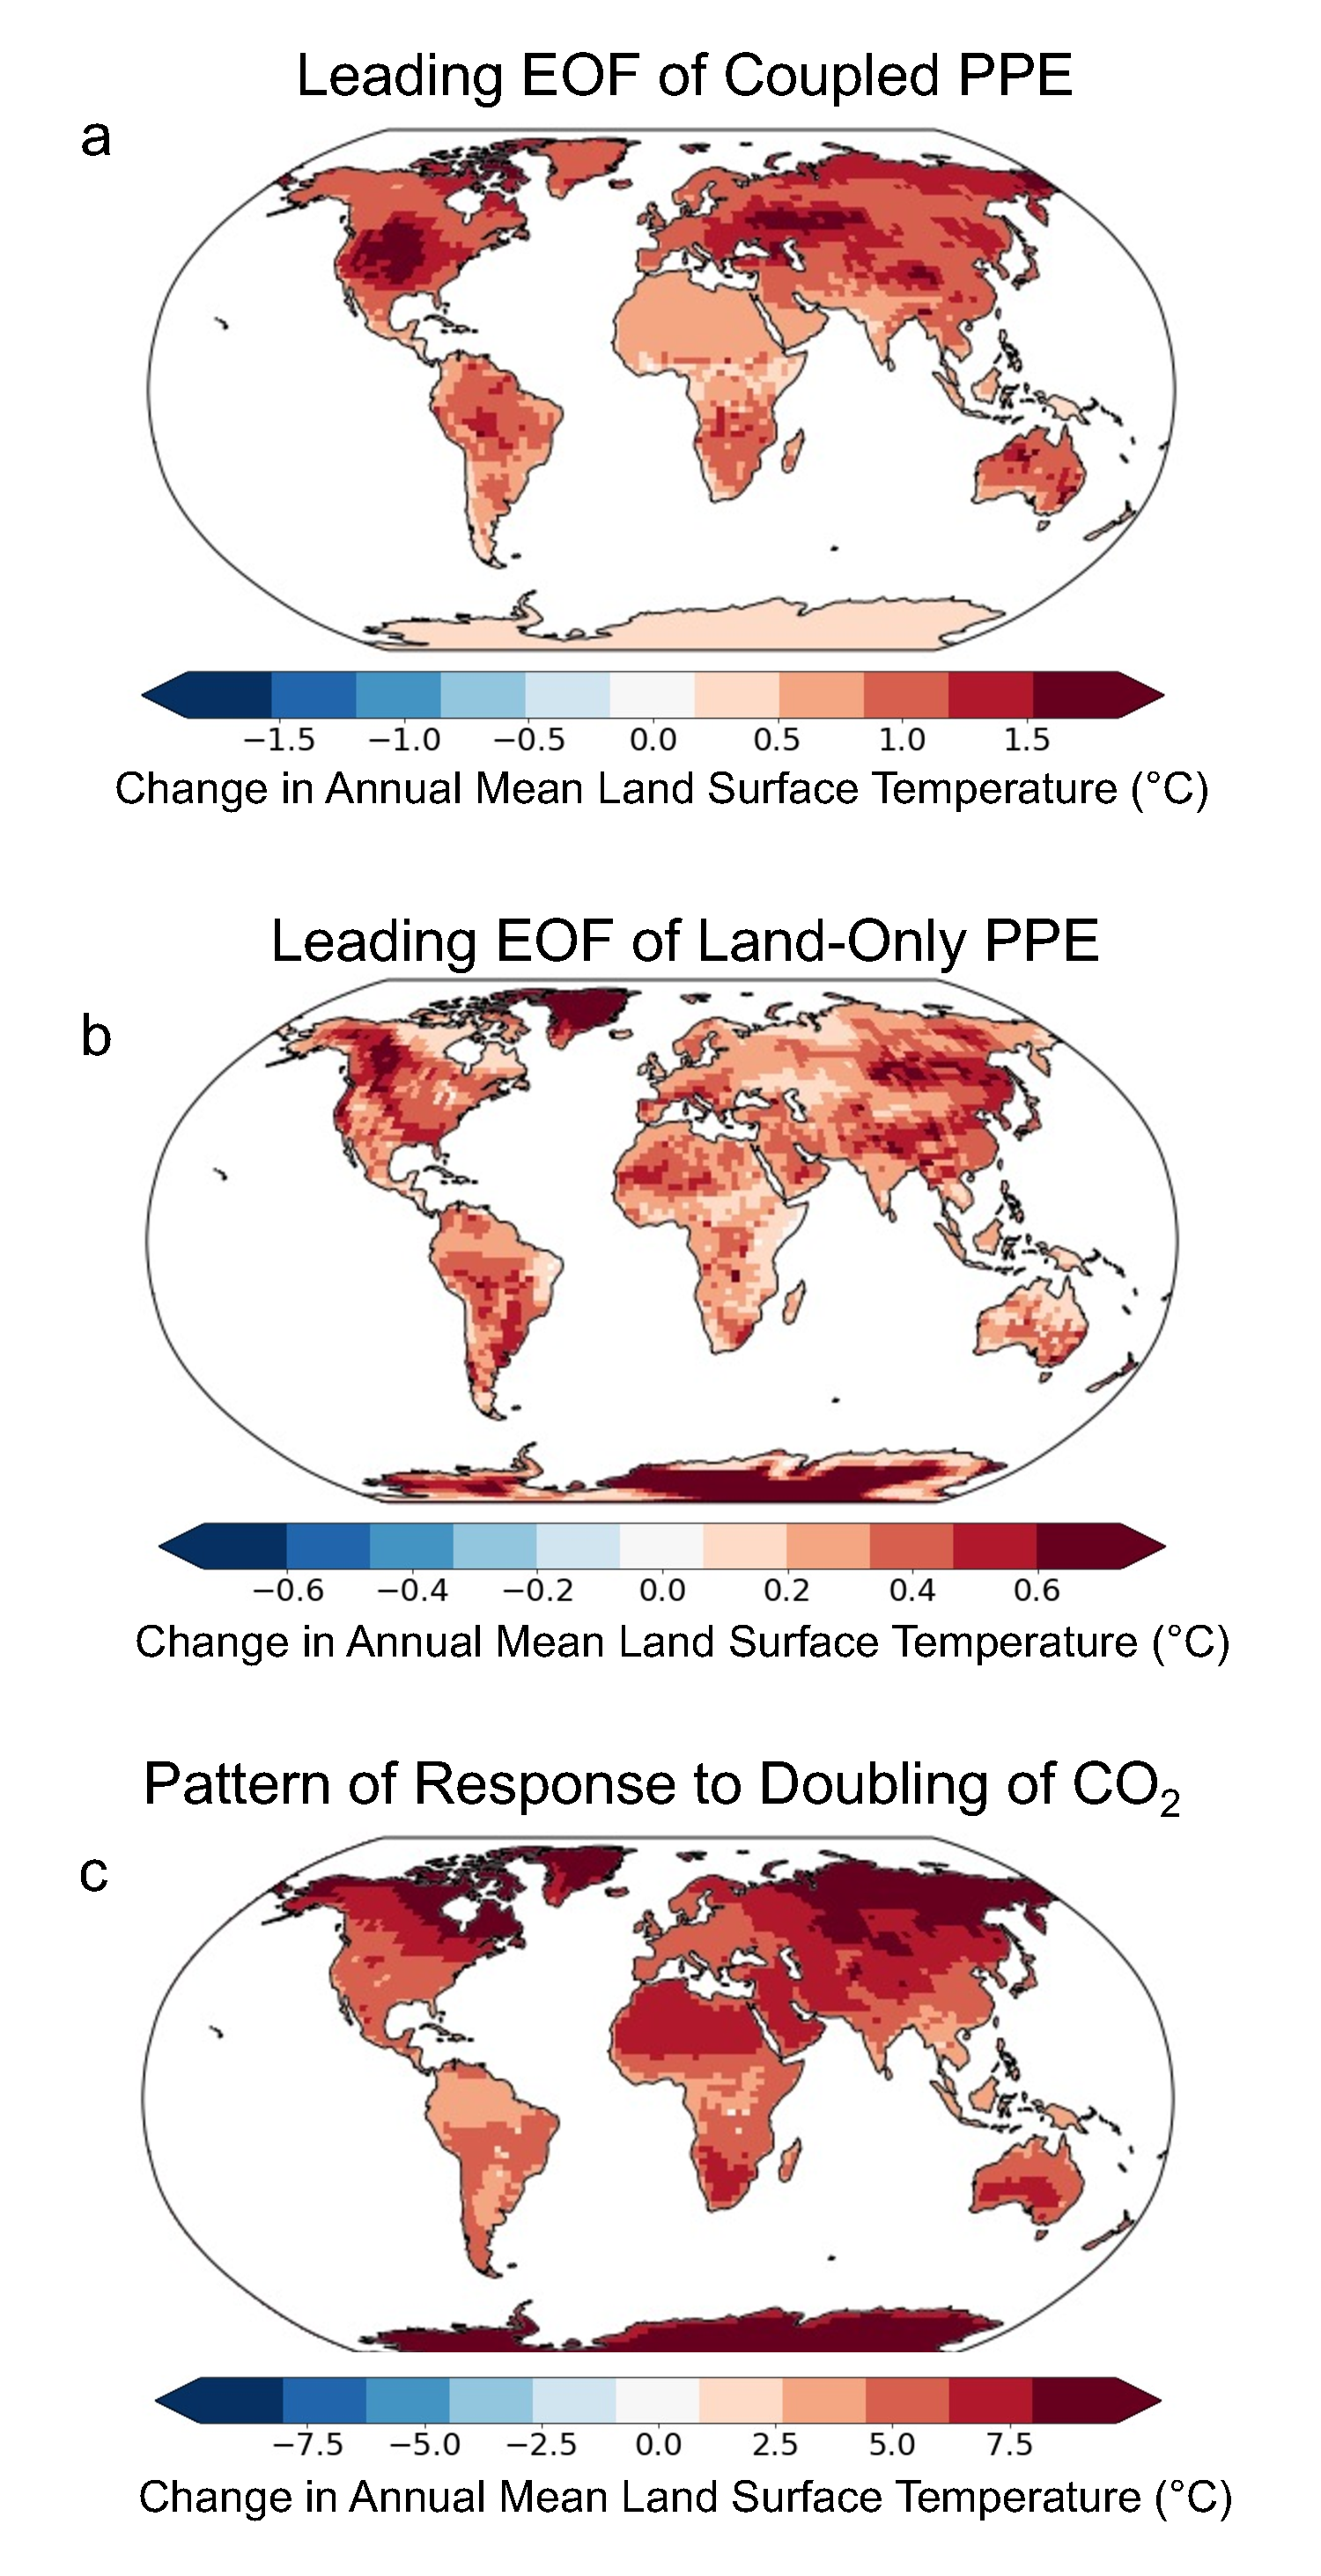
\includegraphics[height=\dimexpr\textheight-80pt\relax]{figs/Figure2.pdf}
\caption{Spatial patterns of annual mean temperature change. The leading EOF of annual mean temperature change across (a) the coupled PPE and (b) the land-only PPE explain 78$\%$ and 65$\%$ of the variance across the coupled and land-only PPEs, respectively. The EOFs are scaled to depict two standard deviations of the variation across the ensemble along that mode of variability. The bottom panel (c) shows the CESM pattern of warming due to a doubling of CO$_2$ (\ref{Text:doubling_CO2}).}
\label{fig:temperature_patterns}
\end{figure}

The dominant coupled PPE temperature pattern is characterized by temperature sensitivity hotspots in the grassland ecosystems of both North America and eastern Europe / central Asia, and larger temperature changes in the Northern hemisphere than the Southern hemisphere. Across the tropics, the temperature response is larger in South America than in tropical Africa or Asia. This pattern resembles the summer temperature response to soil moisture forcing in the Global Land-Atmosphere Climate Experiment (GLACE) experiments \citep{koster_glace_2006, seneviratne_impact_2013} which we discuss further in section 3.3. The hemispheric asymmetry of the land parameter temperature pattern reflects the higher land fraction in the Northern hemisphere, and land perturbations have a larger impact on climate in zonal bands with higher land fraction \citep{lague_terrestrial_2021}, noting that these are for land-only zonal means and thus already take into account zonal variation in land fraction. \cite{fischer_quantifying_2011}’s land PPE also generated larger land temperature changes in the Northern hemisphere than in the Southern hemisphere, but in \citeauthor{fischer_quantifying_2011} high latitude temperature changes were driven mainly by model sensitivity to snow albedo, while in our PPE most parameters drive high latitude temperature changes. Our PPE generated a larger temperature range than \citeauthor{fischer_quantifying_2011}, perhaps due to the fact that \citeauthor{fischer_quantifying_2011} used a flux-corrected slab ocean which can dampen global-scale temperature responses to perturbations \citep{yamazaki_perturbed_2021}.

%% ------------------------------------------------------------------------ 
\subsection{Mean precipitation changes}
We found that terrestrial precipitation is highly sensitive to land parameter choice. Global annual land mean precipitation ranged by about 5$\%$ ($\sigma$= 1$\%$) across our ensemble, and in several regions our PPE drove annual mean precipitation changes of greater than 30$\%$ (Figure ~\ref{fig:precip_changes}a). The same three soil hydrology parameters which most changed global mean temperature—\mintinline{Fortran}{frac_sat_soil_dsl_init}, \mintinline{Fortran}{d_max}, and \mintinline{Fortran}{fff}—also had the largest impact on precipitation. These three hydrology parameters also generated the most extensive spatial coverage of statistically significant annual mean precipitation changes (Figure S\ref{fig:supp_precip_significance_changes}). Across the PPE, less of the land surface experienced statistically significant changes in annual mean precipitation compared to statistically significant changes in mean temperature (Figures S\ref{fig:supp_maps_precip}, S\ref{fig:supp_pct_stat_sig_land}).

Changing parameters drove spatially variable signs of precipitation change, in contrast to mostly consistent signs of temperature change globally (Figure S\ref{fig:supp_pct_stat_sig}). Similarly, while there was a single dominant temperature response pattern across our PPE, the patterns of annual mean precipitation changes were less consistent across ensemble members. The leading EOF of precipitation change explained 48$\%$ of the variance across the PPE (Figure ~\ref{fig:precip_changes}, S\ref{fig:supp_EOF_analysis_Precip}) compared to the 78$\%$ temperature variance explained. This aligns with the fact that precipitation is generally more variable over time than temperature, and some of the variance across the ensemble is likely due to internal variability. Nonetheless, our PPE identified several hotspots where precipitation is the most sensitive to land parameter choice. In particular the North American Great Plains again emerged as a hotspot when considering precipitation changes on both a percentage (Figure ~\ref{fig:precip_changes}) and absolute (Figure S\ref{fig:supp_precip_range}) basis.

\begin{figure}
\centering
\noindent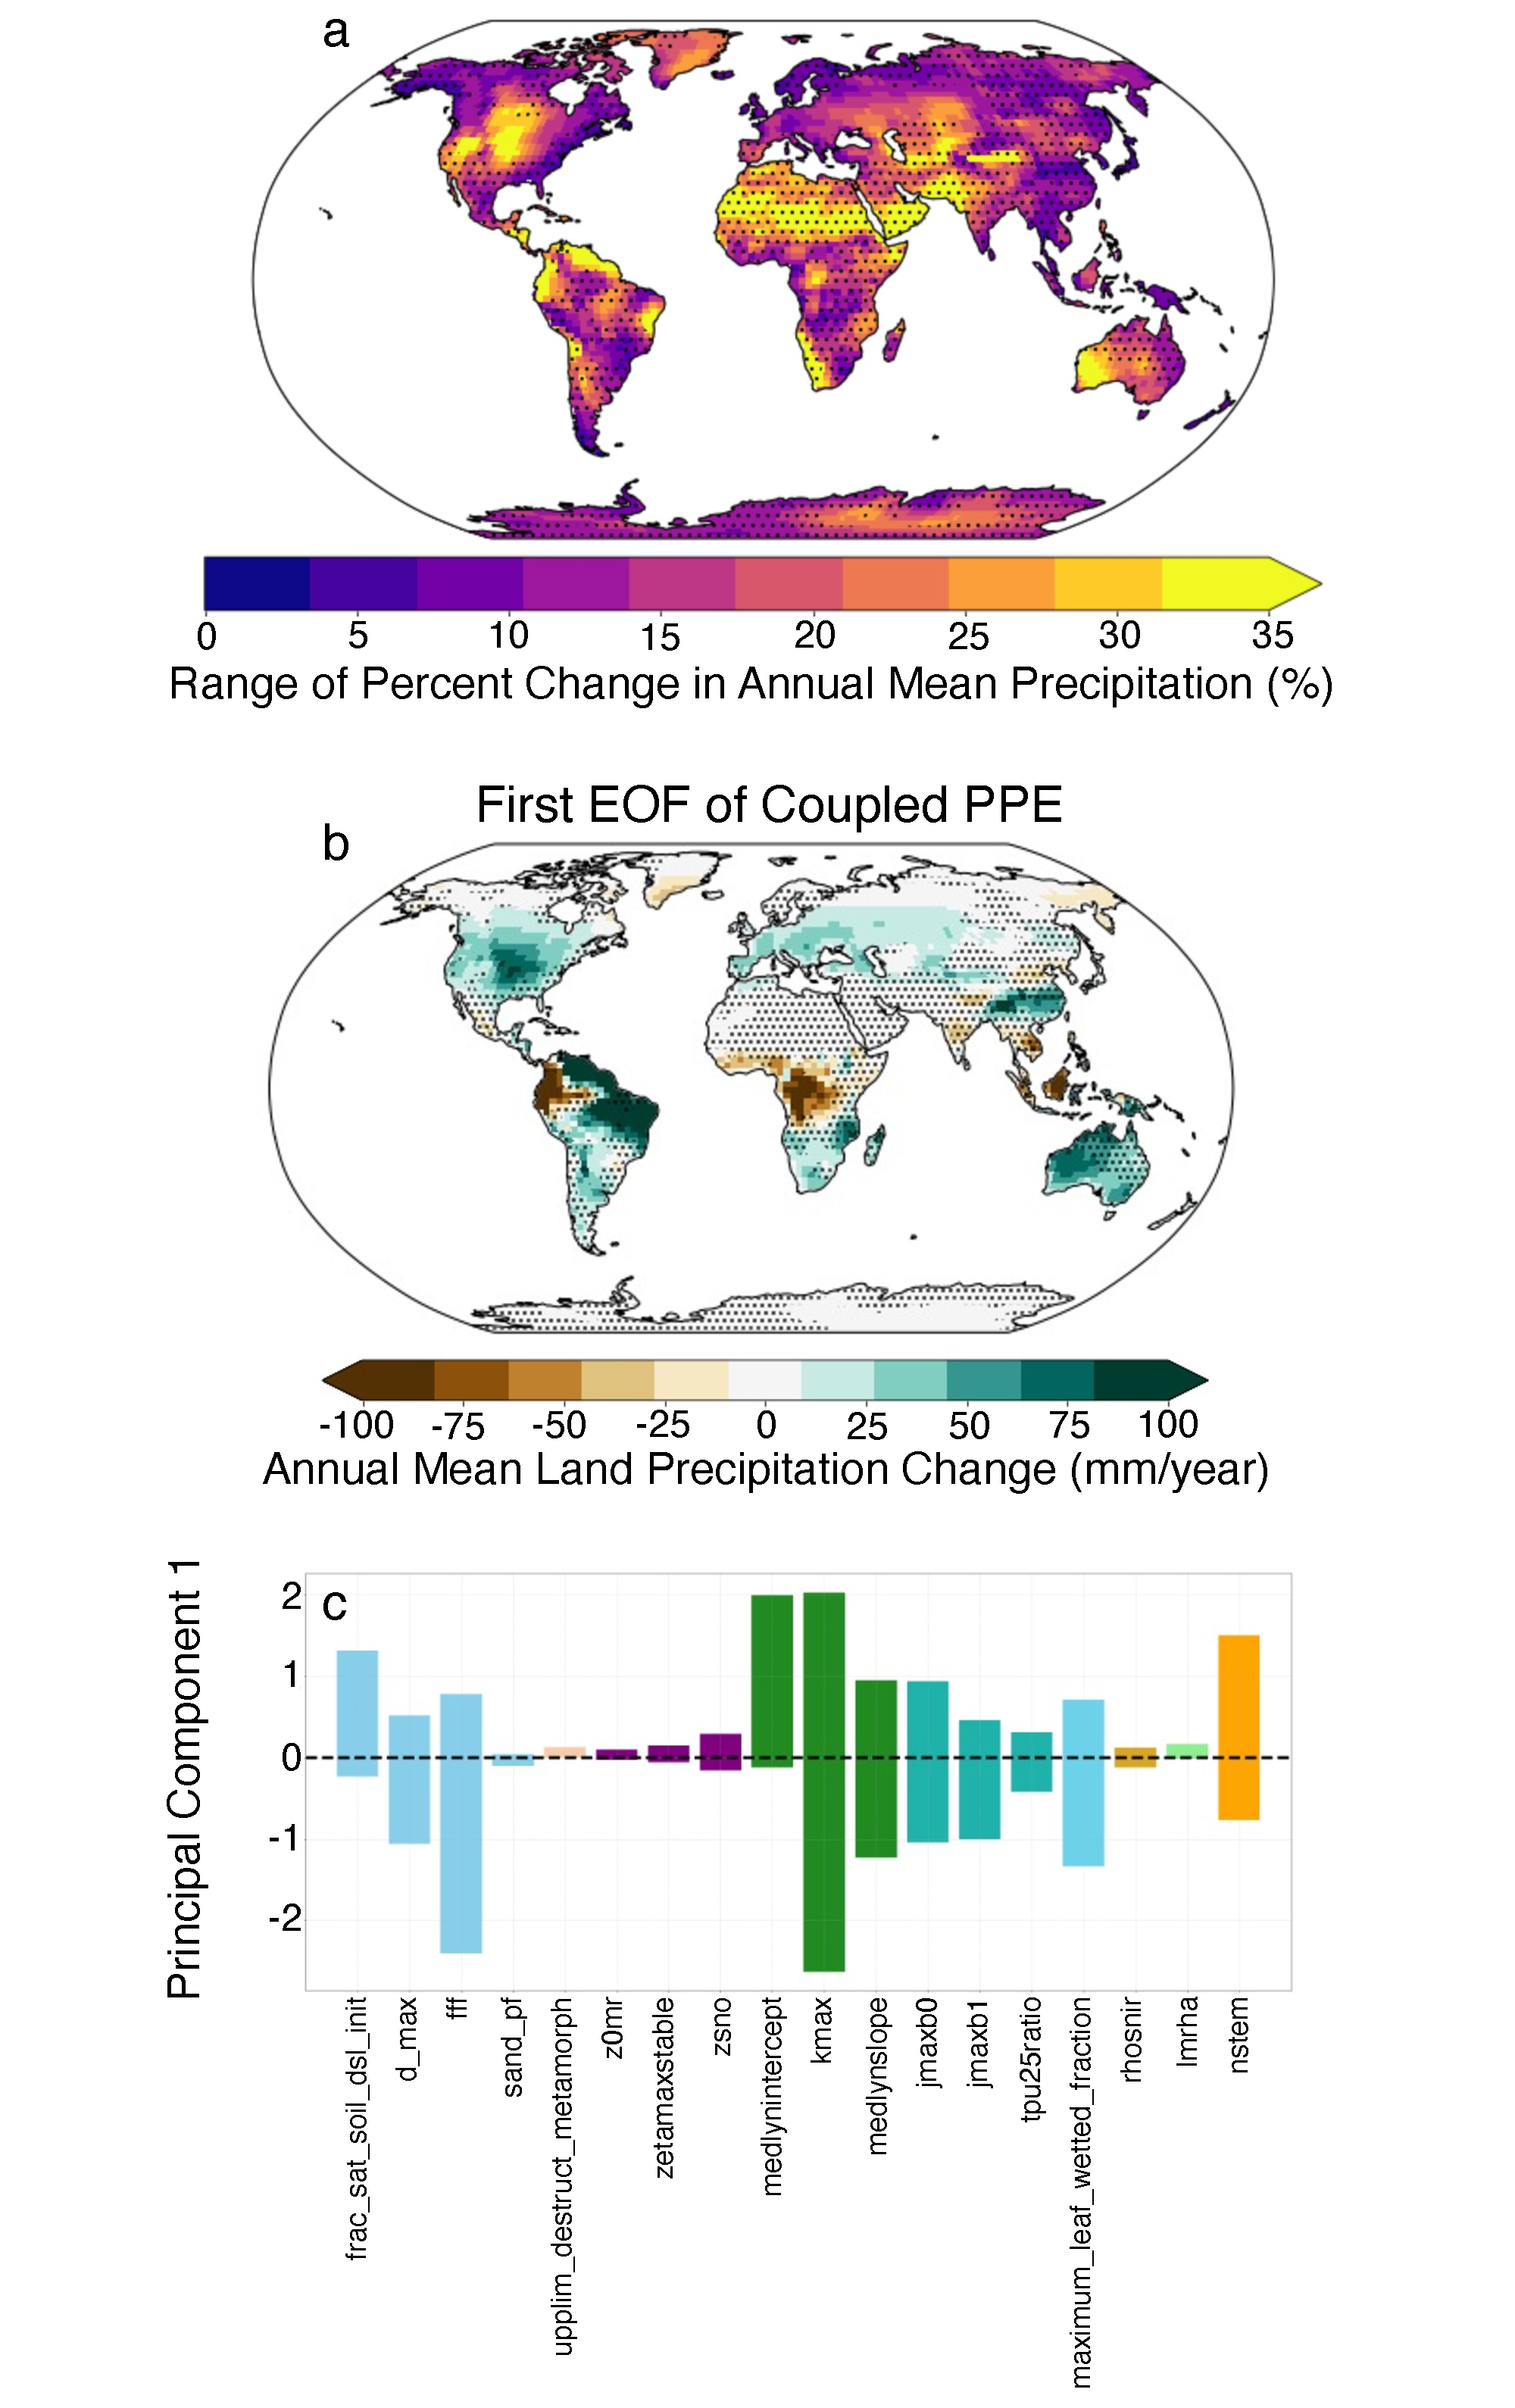
\includegraphics[width=0.8\textwidth]{figs/Figure3.pdf}
\caption{Range of annual mean land precipitation change across the coupled PPE. (a) Map of the range of percent changes in annual mean precipitation across the ensemble. Stippling indicates regions where precipitation changes were not statistically significant for 31 out of 36 ensemble members. (b) First EOF of precipitation changes across the coupled PPE. (c) Principal component 1 across parameters. Colors in (c) indicate parameter category as in Figure \ref{fig:temperature_changes}.}
\label{fig:precip_changes}
\end{figure}

Surprisingly, precipitation in the Great Plains region was not especially sensitive to land parameters in \cite{fischer_quantifying_2011}. However, this region has been identified as a land-atmosphere coupling hotspot due to soil moisture feedbacks in both modeling \citep{koster_glace_2006, santanello_landatmosphere_2018, zheng_impacts_2015} and observational \citep{ferguson_global_2012, abdolghafoorian_validating_2021} studies. Many land-atmosphere studies use metrics that quantify covariances of surface fluxes and the land and atmospheric state on daily timescales. Here we are quantifying how land assumptions influence climate on decadal rather than daily timescales, but this spatial correspondence suggests that changing land parameters may influence long-term climate through mechanisms similar to the soil moisture feedbacks that drive land-atmosphere coupling on daily timescales.


%% ------------------------------------------------------------------------ 
\subsection{Mechanisms through which land parameters influence climate}
Parameters relating to soil hydrology and plant water use drove the largest temperature and precipitation changes in our ensemble (Figure ~\ref{fig:temperature_changes}b, ~\ref{fig:precip_changes}c), highlighting that hydrological processes play a critical role in determining land temperature and precipitation. We note that we purposefully chose parameters across a range of model components and that soil hydrology parameters did not dominate the land-only CLM5 PPE rankings of parameters with the largest impact on global temperature (Figure S\ref{table:supp_param_rankings}), so we did not expect a priori that hydrological processes would dominate the temperature response. We also found that multiple parameters typically evaluated in the context of biogeochemical rather than biogeophysical impacts (e.g., \mintinline{Fortran}{jmaxb0}, the baseline proportion of nitrogen allocated for electron transport; \mintinline{Fortran}{jmaxb1} the response of the electron transport rate to light availability) can still generate large climate responses through biogeophysical pathways, consistent with prior work \citep{smith_biophysical_2017}. We note that the large climate responses reflect both the climate sensitivity to a change in a parameter and the magnitude of the parameter ranges we tested. Parameters that influence boundary layer processes and roughness length drove the smallest global mean temperature changes, but they generated significant local temperature and precipitation changes, particularly over ice sheets and snow-covered regions (Figure S\ref{fig:supp_coupled_Ts_land_maps}).

It is challenging to fully disentangle the pathways through which parameters influence climate, because land parameters alter multiple land surface properties simultaneously. For example, increasing the parameter \mintinline{Fortran}{kmax}, which sets the maximum plant hydraulic conductance, simultaneously changes the land surface evaporative resistance, albedo, and aerodynamic roughness, all of which influence temperature through different mechanisms. Increasing \mintinline{Fortran}{kmax} decreases evaporative resistance by increasing the rate at which plants can transpire water, which decreases land temperatures. Increasing \mintinline{Fortran}{kmax} also decreases plant water stress and increases leaf area, which changes albedo and thereby temperature. Increased photosynthetic rates due to reduced plant water stress also increases vegetation height, which can increase aerodynamic roughness, driving further cooling.

We used multiple linear regression to disentangle the extent to which land precipitation and temperature changes across our coupled PPE are driven by three land surface properties: albedo ($\alpha$), evaporative fraction (EF), and a measure of aerodynamic coupling ($r_a$) (\ref{Text:land_surface properties}). This analysis further emphasizes that evapotranspiration changes dominate the spread in land surface temperature and precipitation responses across our PPE. Changes in evaporative fraction explained the most variance across our ensemble, with albedo playing a secondary role (Figure ~\ref{fig:mechanism_disentangling}). Coupled temperature changes due to changes in aerodynamic coupling were minimal. The dominance of the evapotranspiration mechanism in our PPE may in part be due to the subset of parameters we selected from the 40 top parameters identified based on CLM5-PPE output, but nonetheless our results demonstrate that land parameters’ influence on evapotranspiration is an important (and potentially the dominant) mechanism whereby which land parameters influence the mean climate state.

\begin{figure}
\noindent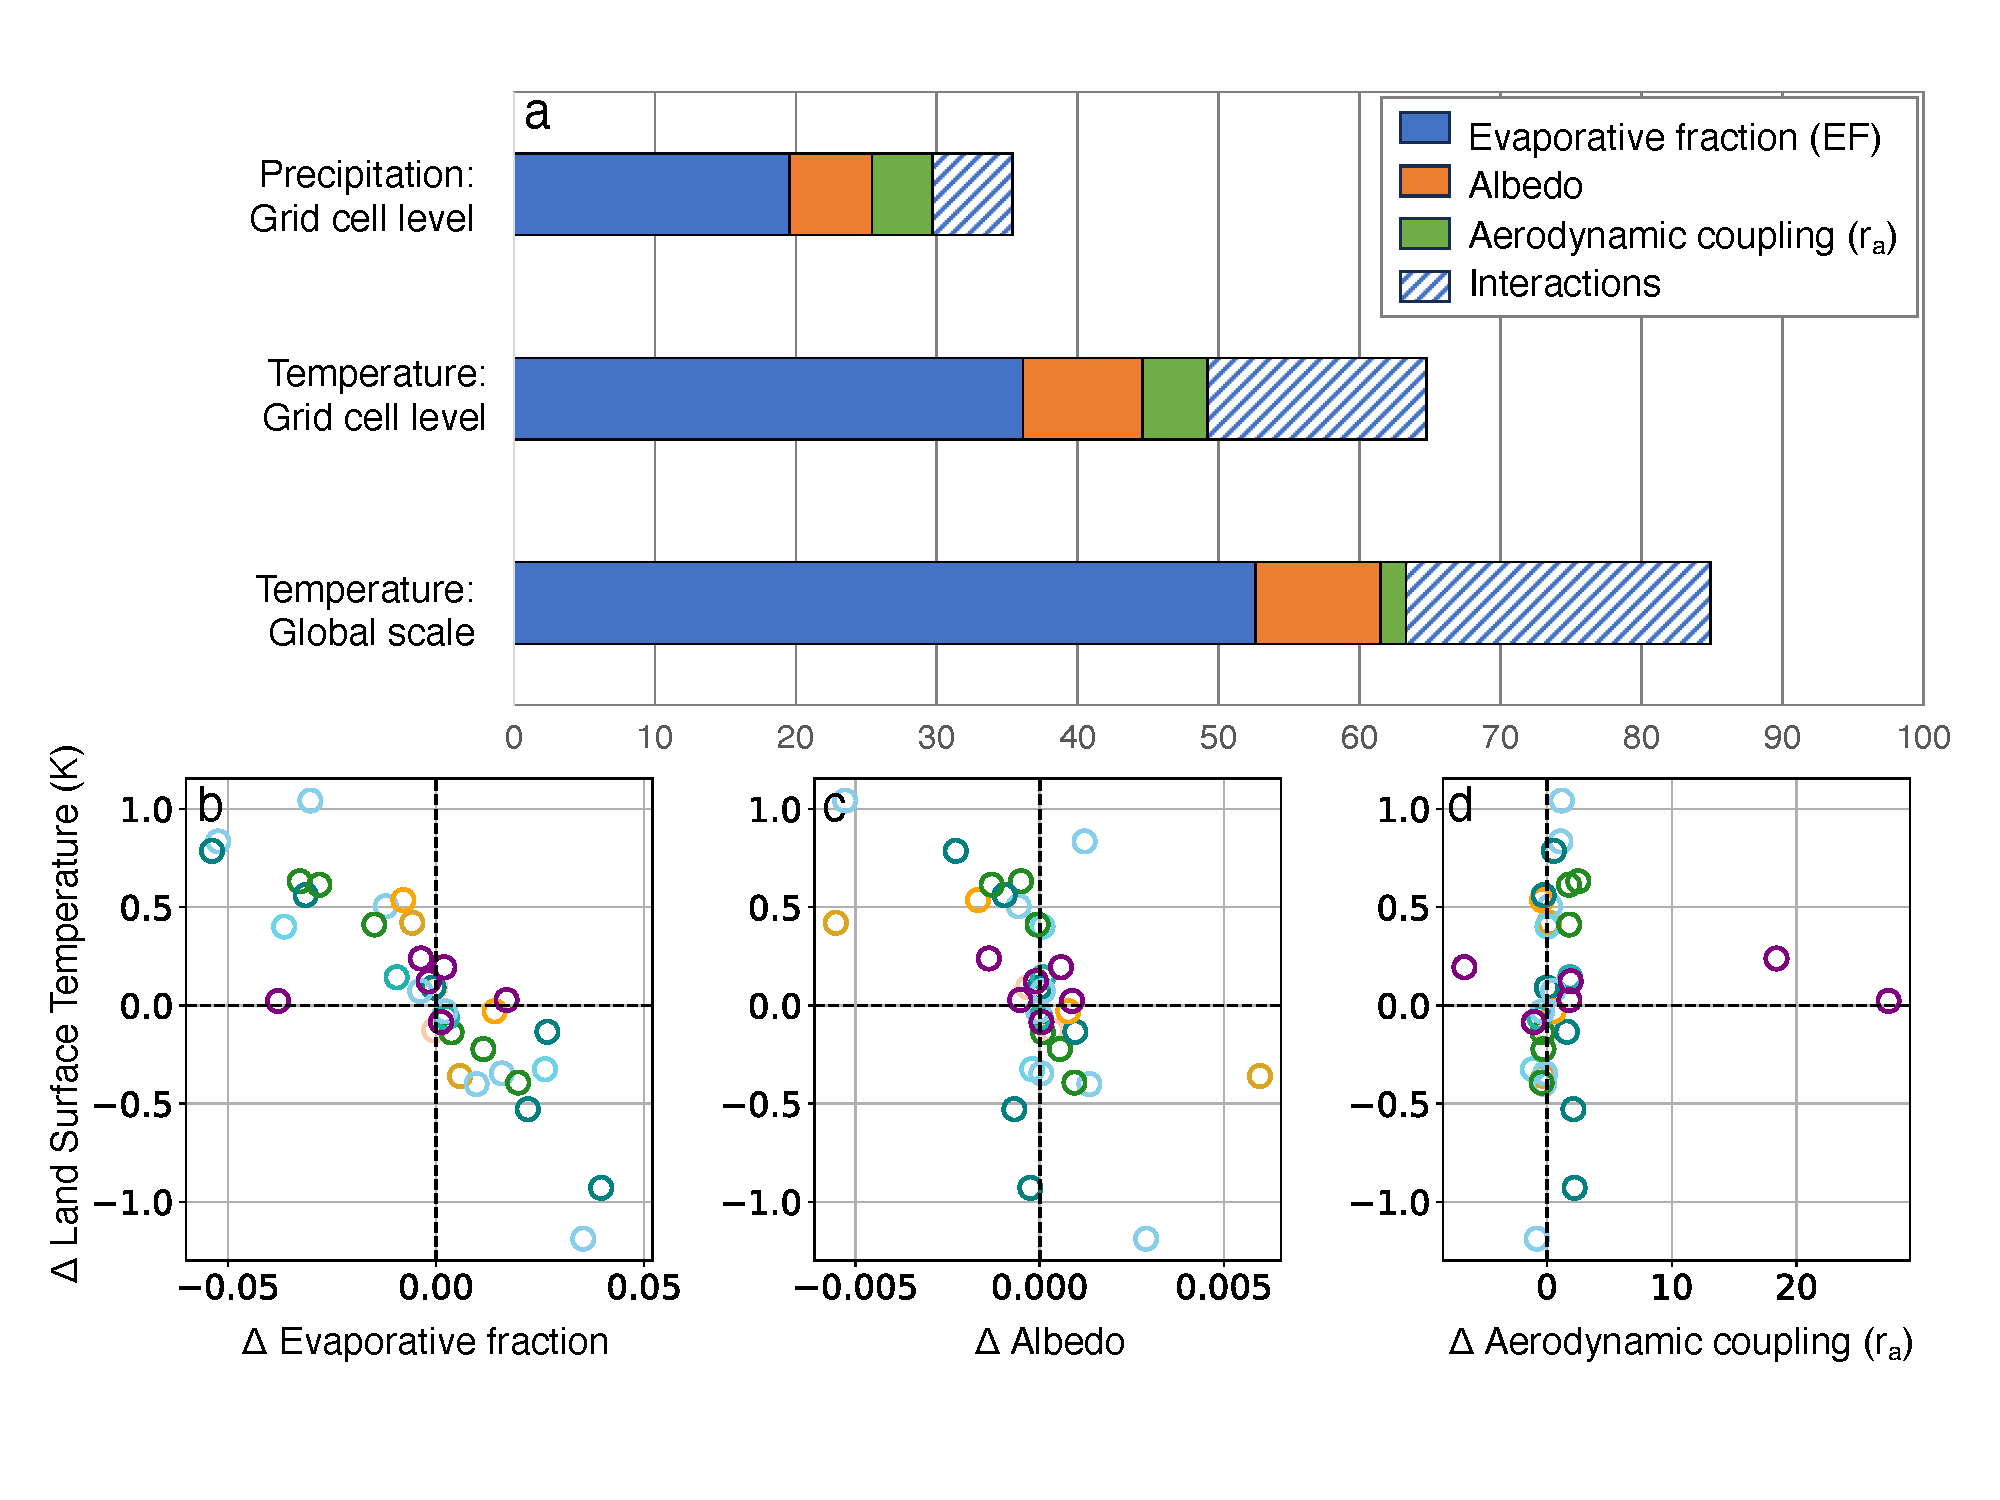
\includegraphics[width=\textwidth]{figs/Figure4.pdf}
\caption{Relationship between land-only surface property changes and coupled land surface climate changes. The top panel (a) shows the percent variance of temperature and precipitation changes explained by each land surface property based on multiple linear regression at the grid cell level, and at the global scale for temperature. Solid colors indicate the marginal additional percentage of variance explained by each land surface property when all other predictors are included, and the hatched bar indicates the percentage variance explained by multiple predictors (i.e. the covariance between predictors). The bottom panel shows the relationships between global mean coupled land surface temperature change and land-only change in (b) evaporative fraction, (c) albedo, and (d) aerodynamic resistance across all ensemble members. Colors indicated parameter category, as in Figure ~\ref{fig:temperature_changes}.}
\label{fig:mechanism_disentangling}
\end{figure}

Further, the dominance of the evapotranspiration mechanism across our ensemble may explain why the leading EOF explains such a high percentage of temperature change variance, and why temperature and precipitation changes are correlated with each other. While we initially designed the PPE to sample multiple processes across CLM’s high-dimensional parameter space (including photosynthesis, snow processes, radiation, etc.), parameters mainly impacted surface climate through changes in evapotranspiration, resulting in an ultimately low-dimensional ensemble of climate responses. We hypothesize that the leading EOFs of temperature and precipitation changes capture the atmospheric response to land evapotranspiration changes, which is supported by the strong correlation between land-only changes in evaporative fraction and the leading coupled temperature and precipitation EOFs (Figure S\ref{fig:supp_EF_EOF_correlation}). The spatial correspondence of mean climate changes between our PPE and GLACE experiments \citep{seneviratne_impact_2013} further supports this interpretation, because in GLACE experiments soil moisture forcing is also influencing climate by modifying turbulent fluxes. However, we note that the climate responses in our PPE are not directly driven by soil moisture changes. Rather, land parameter perturbations influence land evaporative resistance, which directly influences land evapotranspiration independently of any soil moisture change. That land evapotranspiration change (and associated climate feedbacks) can in turn influence soil moisture, but in our experimental design soil moisture changes are an effect or feedback, rather than an external forcing.

It has long been recognized that changes in soil moisture and evaporative resistance can impact climate \citep{shukla_influence_1982,sellers_comparison_1996,seneviratne_impact_2013,lague_separating_2019}, but this is the first study to our knowledge that quantifies how parameter uncertainty associated with terrestrial controls on evapotranspiration impacts mean climate, and compares the impact of the evapotranspiration mechanism to other land surface property changes. For example, the only previous study that quantified the global biogeophysical impact of land parameter uncertainty \citep{fischer_quantifying_2011} did not evaluate the relative impact of evapotranspiration, albedo, and aerodynamic resistance changes on climate. Leveraging the results of the land-only CLM5-PPE enabled us to take a more systematic approach to parameter selection, yielding new insights which may not have emerged had we chosen parameters based on our own assumptions or prior work. This highlights the value of projects that systematically quantify and report parameter uncertainty in land models (e.g. the CLM5 PPE), which we encourage land modeling groups to incorporate as a standard part of model development and documentation efforts. This study also underscores the importance of developing better observational constraints for land parameters which influence evapotranspiration.

%% ------------------------------------------------------------------------ 
\section{Conclusions}
This study highlights a large and underappreciated impact of land processes in determining the mean climate state. We used a PPE to quantify the biogeophysical impact of land parameters on terrestrial climate. We found that land parameters can substantially impact mean temperature and precipitation, primarily through parameters’ influence on evapotranspiration, and that uncertainty associated with soil hydrology and plant water use parameters drive the largest spread in the mean climate state. Uncertainty in land models' representation of land surface fluxes stems from multiple sources: internal variability, model structure, and model parameters. This study focuses on the effect of land parametric uncertainty, but our results demonstrate the importance of land process uncertainty more generally because both model structure and parameters control the land surface properties (e.g., evaporative resistance) that ultimately influence climate.

Land processes’ influence on climate means that biases in land models can contribute to biases in ESM climatology. Biases in land evapotranspiration have been invoked as possible drivers for several persistent ESM biases \citep[e.g., the central United States warm and dry summer biases,][]{klein_diagnosis_2006, cheruy_role_2014, williams_land-atmosphere_2016, lin_causes_2017, morcrette_introduction_2018, zhang_causes_2018, ma_causes_2018, mueller_systematic_2014}, and this work directly shows how land assumptions can influence the mean climate at regional and global scales, demonstrating the importance of including land perspectives in the assessments of model biases. Additionally, this study underscores that land processes primarily discussed in the context of carbon cycle uncertainty (e.g. photosynthesis) can have large biogeophysical impacts on the physical climate, in addition to their influence on atmospheric CO$_2$ concentration.

There has been a concerted effort across climate modeling centers to create ‘digital twins’ of the Earth \citep[e.g., ][]{voosen_europe_2020, li_big_2023} by increasing climate model resolution, thereby enabling direct modeling of fine-scale atmospheric processes such as convection that are subgrid-scale parameterizations in coarser scale models \citep{betancourt_are_2022}. While increased resolution will likely diminish biases associated with some atmospheric processes, increased resolution does less to improve land process representation because many land processes occur at molecular to hillslope scales and therefore will continue to require subgrid parameterizations \citep{fisher_perspectives_2020,reichstein_deep_2019,balaji_are_2022}. Further, finite computational resources imply tradeoffs between increasing resolution and the number of ensembles to quantify parameter uncertainty and calibrate models. If atmospheric-focused model advancements are not accompanied by efforts to improve land models, land parameter uncertainty may remain a persistent driver of climatological uncertainty and biases, even in the next generation of high-resolution climate models. Recognizing that land process uncertainty influences climate also presents an opportunity for model improvement. The climate modeling community has historically devoted more effort to atmospheric uncertainty than to land uncertainty \citep{hourdin_art_2017}, and we hypothesize that committing comparable resources to land parameter calibration could drive rapid improvements in model representation of present-day climate.

By demonstrating that land parameters influence the mean climate state, we hope that this study will stimulate further research into the climate impacts of land process uncertainty by a broader geophysical research community. In particular, our results suggest there is potential for land parameter uncertainty to influence the sensitivity of land temperature trends to historical and future climates, and we plan to test this in future work. Because the evaporative fraction influences how much the land surface warms in response to radiative forcing, we hypothesize that changing parameters that influence the baseline evaporative fraction will influence the modeled trajectory of land surface temperatures under increasing greenhouse gas concentrations, even if the evaporative fraction were to remain constant over time. Furthermore, land processes influence how the evaporative fraction changes over time, for example due to plant physiological responses to CO$_2$ \citep{lemordant_critical_2018}. Quantifying how land parameter uncertainty influences future land temperature trajectories should be a high research priority.

While land modeling has substantially expanded beyond its initial scope of providing lower atmospheric boundary conditions into its own subdiscipline and research community, land models’ continued role as atmospheric boundary conditions means that a broader climate science community must engage with land processes (and uncertainty therein) in order to understand and model the physical climate system.
%% ------------------------------------------------------------------------ 
\section{Open Research}
The model output used in this paper will be deposited in the Dryad Digital Repository (with a DOI) once the paper is accepted with revisions. This data is currently archived on servers at the National Center for Atmospheric Research. Code used to run simulations and analyze model output are available at \url{https://github.com/czarakas/coupled_PPE}.
%% ------------------------------------------------------------------------ 
\acknowledgments
CMZ was supported by the U.S. Department of Energy (DOE) Computational Science Graduate Fellowship (DE-SC0020347). The DOE Office of Biological and Environmental Research Regional and Global Model Analysis Program supported ALSS, AL, and CMZ (DE-SC0021209); KD (DE-SC0022070); and CDK and DML (DE-AC02-05CH11231 through the RUBISCO SFA). The National Science Foundation (NSF) also supported ALSS and CMZ (AGS-1553715) and KD (NSF IA 1947282). The CESM project is supported primarily by the NSF. This material is based upon work supported by the National Center for Atmospheric Research, which is a major facility sponsored by the NSF under Cooperative Agreement No. 1852977. The Computational and Information Systems Laboratory at NCAR provided computing and data storage resources, including the Cheyenne supercomputer (\url{https://doi.org/10.5065/D6RX99HX}). We thank all scientists, software engineers, and administrators who contributed to CESM2's development.
%% ------------------------------------------------------------------------ 
%TC:ignore
\bibliography{PPE_refs}
%TC:endignore
\end{document}
